\let\negmedspace\undefined
\let\negthickspace\undefined
%\RequirePackage{amsmath}
\documentclass[journal,12pt,twocolumn]{IEEEtran}
\usepackage[utf8]{inputenc}
\usepackage{graphicx}
\usepackage{amsmath}
\usepackage{amsfonts}
\usepackage{amssymb}
\usepackage{enumitem}
\usepackage{mathtools}
\usepackage[breaklinks=false]{hyperref}
\usepackage{listings}
\usepackage{calc}

\newcommand{\BEQA}{\begin{eqnarray}}
\newcommand{\EEQA}{\end{eqnarray}}
\newcommand{\define}{\stackrel{\triangle}{=}}
\bibliographystyle{IEEEtran}
%\bibliographystyle{ieeetr}
\let\vec\mathbf
\providecommand{\brak}[1]{\ensuremath{\left(#1\right)}}
\newcommand{\myvec}[1]{\ensuremath{\begin{pmatrix}#1\end{pmatrix}}}
\newcommand{\mydet}[1]{\ensuremath{\begin{vmatrix}#1\end{vmatrix}}}
\newcommand{\question}{\noindent \textbf{Question: }}
\newcommand{\solution}{\noindent \textbf{Solution: }}
\title{Probability and Random Variables\\Assignment 1}
\author{Mayuri Chourasia\\BT21BTECH11001}
\date{}
\begin{document}
% make the title area
\maketitle
\question
\begin{enumerate}[label=]
\item The vertices of a $\triangle$ ABC are \vec{A}(3,8), \vec{B}(-1,2) and \vec{C}(6,-6). Find:
\begin{enumerate}
    \item Slope of \vec{BC}
    \item Equation of a line perpendicular to \vec{BC} and passing through \vec{A}
\end{enumerate}
\end{enumerate}
\solution
\begin{enumerate}
	\begin{figure}[h]
	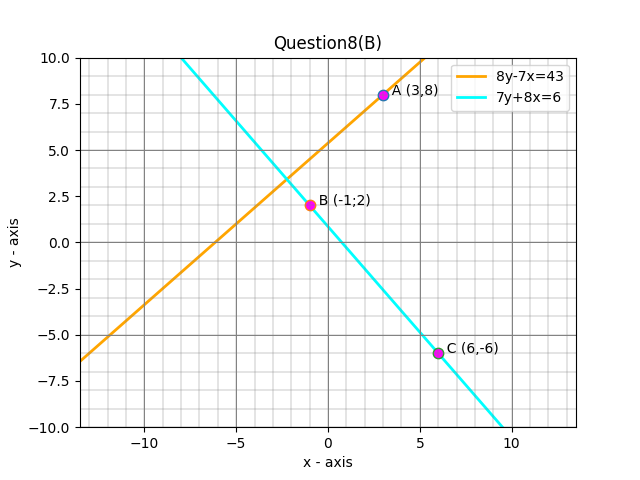
\includegraphics[width=\columnwidth]{Graph(PNG_file).png}
	\caption{Plot showing $\triangle$ABC, line BC and line perpendicular to BC.}
	\label{Fig1}
	\end{figure}
\item Let $\vec{A}, \vec{B}, \vec{C}$ be the points vectors.
	\begin{align}
		\vec{A} = \myvec{3 \\ 8} ,
		\vec{B} = \myvec{-1 \\ 2}  ,
		\vec{C} = \myvec{6 \\ -6}
	\end{align}
	$\therefore$ The direction vector of $BC$ is,
    \begin{align}
    &\vec{m} = \vec{C} - \vec{B}
    \\
	\implies &\vec{m} = \myvec{6 \\ -6} - \myvec{-1 \\ 2}
	\\
	\implies &\vec{m} = \myvec{7 \\ -8}
    \end{align}
    We know that, if the direction vector of a line is represented by a matrix \vec{m}=\myvec{d_1\\d_2} then the slope for the same can be represented by $\brak{\frac{d_2}{d_1}}$.\\
    \medskip\\
    \textbf{Therefore in this case the slope of line BC can be given as:}
    \begin{align}
        slope=\frac{-8}{7}
    \end{align}
    \medskip\\
\item Now, let $n_{BC}$ be the normal vector of the line BC, hence we know that;
    \begin{align}
	&\vec{m}^{\top}\vec{n_{BC}} = 0
	\\
	\implies &\myvec{7 & -8}\vec{n_{BC}} = 0
	\\
	\implies &\vec{n_{BC}} = \myvec{8 \\ 7}
	\\
	\implies &\vec{n_{BC}^{\top}} = \myvec{8 & 7}
    \end{align}
     Let L be the line that passes through A and is perpendicular to BC, and let $n_L$ be the normal vector of the line L, in such a case we can say that;
     \begin{align}
	&\vec{n_{BC}^{\top}} \vec{n_L} = 0
	\\
	\implies &\myvec{8 & 7}\vec{n_L} = 0
	\\
	\implies &\vec{n_L} = \myvec{7 \\ -8}
	\\
	\implies &\vec{n_L}^{\top} = \myvec{7 & -8}
    \end{align}
    The normal equation of the line L is given by, 
    \begin{align}
	&\vec{n_L}^{\top} \brak{\vec{X}-\vec{A}} = 0
	\\
	\implies &\myvec{7 & -8}\brak{\vec{X} - \myvec{3 \\ 8}}= 0
	\\
	\implies &\myvec{7 & -8}\vec{X}- \myvec{7 & -8}\myvec{3\\8}= 0
	\\
	\implies &\myvec{7 & -8}\vec{X} = \brak{-43}
    \end{align}
    \textbf{Thus, line L $\equiv \myvec{7 & -8}\vec{X} = \brak{-43}$}
\end{enumerate}
\end{document} 
